\documentclass[tikz]{standalone}
\usepackage{libertinus-otf}
\usepackage{unicode-math, amsmath}
\usepackage{tikz}
\begin{document}
	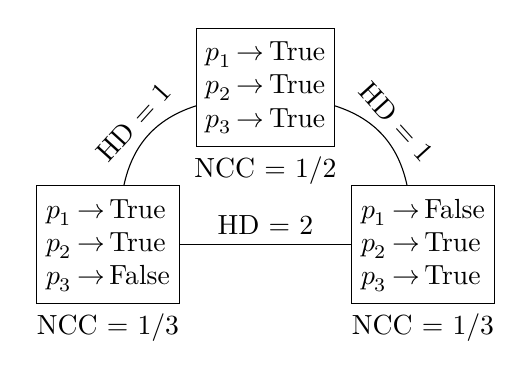
\begin{tikzpicture}
		\node (pos1) [draw, label={below:NCC = 1/2}] {\begin{tabular}{@{}l@{\,$\rightarrow$\,}l@{}}
				$p_1$ & True\\
				$p_2$ & True\\
				$p_3$ & True\\
		\end{tabular}};
		\node (pos2) at (2,-2) [draw, label={below:NCC = 1/3}] {\begin{tabular}{@{}l@{\,$\rightarrow$\,}l@{}}
				$p_1$ & False\\
				$p_2$ & True\\
				$p_3$ & True\\
		\end{tabular}};
		\node (pos3) at(-2,-2) [draw, label={below:NCC = 1/3}] {\begin{tabular}{@{}l@{\,$\rightarrow$\,}l@{}}
				$p_1$ & True\\
				$p_2$ & True\\
				$p_3$ & False\\
		\end{tabular}};
		\draw (pos1) to[bend left] node[above,sloped] {HD = 1} (pos2);
		\draw (pos1) to[bend right] node[above,sloped] {HD = 1} (pos3);
		\draw (pos2) to node[above,sloped] {HD = 2} (pos3);		
	\end{tikzpicture}
\end{document}